% Options for packages loaded elsewhere
\PassOptionsToPackage{unicode}{hyperref}
\PassOptionsToPackage{hyphens}{url}
\documentclass[
]{article}
\usepackage{xcolor}
\usepackage[margin=1in]{geometry}
\usepackage{amsmath,amssymb}
\setcounter{secnumdepth}{-\maxdimen} % remove section numbering
\usepackage{iftex}
\ifPDFTeX
  \usepackage[T1]{fontenc}
  \usepackage[utf8]{inputenc}
  \usepackage{textcomp} % provide euro and other symbols
\else % if luatex or xetex
  \usepackage{unicode-math} % this also loads fontspec
  \defaultfontfeatures{Scale=MatchLowercase}
  \defaultfontfeatures[\rmfamily]{Ligatures=TeX,Scale=1}
\fi
\usepackage{lmodern}
\ifPDFTeX\else
  % xetex/luatex font selection
\fi
% Use upquote if available, for straight quotes in verbatim environments
\IfFileExists{upquote.sty}{\usepackage{upquote}}{}
\IfFileExists{microtype.sty}{% use microtype if available
  \usepackage[]{microtype}
  \UseMicrotypeSet[protrusion]{basicmath} % disable protrusion for tt fonts
}{}
\makeatletter
\@ifundefined{KOMAClassName}{% if non-KOMA class
  \IfFileExists{parskip.sty}{%
    \usepackage{parskip}
  }{% else
    \setlength{\parindent}{0pt}
    \setlength{\parskip}{6pt plus 2pt minus 1pt}}
}{% if KOMA class
  \KOMAoptions{parskip=half}}
\makeatother
\usepackage{longtable,booktabs,array}
\usepackage{caption}
\captionsetup[table]{skip=6pt}
\newcounter{none} % for unnumbered tables
\usepackage{calc} % for calculating minipage widths
% Correct order of tables after \paragraph or \subparagraph
\usepackage{etoolbox}
\makeatletter
\patchcmd\longtable{\par}{\if@noskipsec\mbox{}\fi\par}{}{}
\makeatother
% Allow footnotes in longtable head/foot
\IfFileExists{footnotehyper.sty}{\usepackage{footnotehyper}}{\usepackage{footnote}}
\makesavenoteenv{longtable}
\usepackage{graphicx}
\makeatletter
\newsavebox\pandoc@box
\newcommand*\pandocbounded[1]{% scales image to fit in text height/width
  \sbox\pandoc@box{#1}%
  \Gscale@div\@tempa{\textheight}{\dimexpr\ht\pandoc@box+\dp\pandoc@box\relax}%
  \Gscale@div\@tempb{\linewidth}{\wd\pandoc@box}%
  \ifdim\@tempb\p@<\@tempa\p@\let\@tempa\@tempb\fi% select the smaller of both
  \ifdim\@tempa\p@<\p@\scalebox{\@tempa}{\usebox\pandoc@box}%
  \else\usebox{\pandoc@box}%
  \fi%
}
% Set default figure placement to htbp
\def\fps@figure{htbp}
\makeatother
\setlength{\emergencystretch}{3em} % prevent overfull lines
\providecommand{\tightlist}{%
  \setlength{\itemsep}{0pt}\setlength{\parskip}{0pt}}
% Course-specific text for the shared PDF theme. Must be listed BEFORE
% ../../_syllabus-template/syllabus-preamble.tex in the YAML in_header.
\newcommand{\courseName}{Democracy's Data}
\newcommand{\courseTerm}{84-355 · Fall 2026}
% ============================================================
% Lab-brief PDF theme — a wider variant of the syllabus PDF theme.
% Print counterpart to brief.css.
%
% syllabus-preamble.tex sets a 4.6in text block with a 1.8in margin
% column, which is right for a reference document. A brief is carried
% by figures, and its figures come off the R device 6.3-6.9in wide.
% At 4.6in the wide ones were scaled to 67-73% and the paired
% cartograms stopped working: 51 state abbreviations below print
% legibility. This file widens the page and stops the scaling.
%
% Nothing in syllabus-preamble.tex is modified. Everything below is
% either a re-issue (geometry) or a layer on top.
%
% USE (from F26/labs/<lab>/, i.e. four levels below _teaching/):
%
%   pdf_document:
%     latex_engine: xelatex
%     includes:
%       in_header:
%         - ../../course-meta.tex
%         - ../../../../_syllabus-template/brief-preamble.tex
%
% course-meta.tex MUST come first. syllabus-preamble.tex declares the
% running head with \providecommand{\courseName}{\@title}; if the
% course file has already defined \courseName the \providecommand is a
% no-op and the head reads DEMOCRACY'S DATA. Drop it and \@title takes
% over, and a brief's title is a 45-character sentence set in 8pt caps
% across the top of every page. Nothing below changes that mechanism —
% the include order is the whole of it.
%
% Listing syllabus-preamble.tex explicitly in in_header, between
% course-meta.tex and this file, also works: the guard below sees it
% is already loaded and does not load it twice.
% ============================================================

% ---- pull in the shared theme ------------------------------
% pandoc pastes in_header files into the preamble rather than \input-ing
% them, so this file cannot know where it was pasted from. Try the
% depths a course actually uses, and no-op if the YAML already listed
% syllabus-preamble.tex ahead of us (\ddfullwidth is its fingerprint).
\makeatletter
\newif\ifdd@basefound \dd@basefoundfalse
\@ifundefined{ddfullwidth}{%
  \def\dd@trybase#1{%
    \ifdd@basefound\else
      \IfFileExists{#1syllabus-preamble.tex}{%
        \dd@basefoundtrue
        \input{#1syllabus-preamble.tex}%
      }{}%
    \fi}%
  \dd@trybase{../../../../../_syllabus-template/}% labs/<NN-part>/<lab>/ (usual)
  \dd@trybase{../../../../_syllabus-template/}%  labs/<lab>/   (unfiled chapters)
  \dd@trybase{../../../_syllabus-template/}%     labs/
  \dd@trybase{../../_syllabus-template/}%        course root
  \dd@trybase{../_syllabus-template/}%
  \dd@trybase{}%                                 same directory
  \ifdd@basefound\else
    \@latex@error{brief-preamble.tex could not find syllabus-preamble.tex.
      List it in the YAML in_header, before this file}\@ehd
  \fi
}{\dd@basefoundtrue}
\makeatother

% ---- page ---------------------------------------------------
% Re-issued, not edited in place. geometry takes the last word, so
% naming only what changes leaves left/top/bottom/headheight as the
% syllabus set them.
%
%   left 1.0in | text 5.30in | sep 0.30in | margin 1.50in | 0.40in
%   \--------------------- 8.5in letter ---------------------/
%
% right = 2.2in is the measure decision: 5.3in of text instead of
% 4.6in. marginparwidth comes down from 1.8in to 1.5in to pay for it.
% That is not a rounding choice — \ddfullwidth is textwidth + sep +
% marginparwidth, and everything the syllabus theme sets to
% \ddfullwidth (the title rule, the stat grid, and every longtable)
% grows with it. At the inherited 1.8in the full width would be 7.4in
% and those blocks would finish 0.1in from the paper edge, off the
% printable area of most printers. At 1.5in it is 7.1in, finishing
% 0.4in in — still wide, still on the paper.
\geometry{
  right          = 2.2in,
  marginparwidth = 1.5in
}

% \ddfullwidth is measured \AtBeginDocument by syllabus-preamble.tex.
% Re-measure after it, so the value reflects the geometry above however
% geometry chooses to apply itself. Registered second, so it runs second.
\AtBeginDocument{%
  \setlength{\ddfullwidth}{\dimexpr\textwidth+\marginparsep+\marginparwidth\relax}%
}

% Same problem, other file: syllabus-preamble.tex runs the red head rule
% across the margin column with
%   \fancyhfoffset[R]{\dimexpr\marginparsep+\marginparwidth\relax}
% and fancyhdr freezes that offset the moment it is issued — under the
% syllabus's 1.8in margin, i.e. 2.1in. Left alone, the rule would finish
% 0.3in past the content it is supposed to cap. Re-issue it late, once
% geometry has settled, so head rule and \ddfullwidth end on the same
% vertical.
\AtBeginDocument{%
  \fancyhfoffset[R]{\dimexpr\marginparsep+\marginparwidth\relax}%
}

% ---- figures at their natural size --------------------------
% The whole point of the file.
%
% pandoc's template defines
%   \def\maxwidth{\ifdim\Gin@nat@width>\linewidth\linewidth\else\Gin@nat@width\fi}
% and then \setkeys{Gin}{width=\maxwidth,...}, so every graphic is
% clamped to the text column. The briefs' figures are 6.3-6.9in wide,
% which is why a 4.6in column shrank them to two-thirds.
%
% Clamp at \ddfullwidth (7.1in) instead. This is a template default,
% not a per-figure override: figures narrower than the full width are
% untouched — the tile cartogram comes off the device at 4.21in and
% stays at 4.21in — and the wide ones run out into the margin column,
% which is where Tufte puts wide material anyway and which is dead
% space beside a figure regardless.
%
% Measured on electoral-map-brief, six figures, natural -> placed:
%   6.278 -> 6.278   4.208 -> 4.208   6.750 -> 6.750
%   6.319 -> 6.319   6.736 -> 6.736   6.847 -> 6.847
% All six at 100%. The same six at the syllabus's 4.6in measure sat
% at 67-73% except the cartogram, which was already narrow enough.
%
% CAVEAT, and it is the one thing to watch in a brief that uses the
% margin apparatus: a figure occupying the margin column and a
% \marginpar raised at the same vertical position do not know about
% each other, and LaTeX will not move either of them. The same is
% already true of the widened longtables in syllabus-preamble.tex, so
% this is not a new hazard, but it is a wider one. If a brief has both
% wide figures and sidenotes, keep the notes away from the figures —
% attach them to the paragraph before or the paragraph after.
%
% Deferred to \AtBeginDocument for two reasons: pandoc's \def comes
% later in the preamble than in_header on some template versions, and
% \ddfullwidth has no value until then.
\makeatletter
\AtBeginDocument{%
  \def\maxwidth{%
    \ifdim\Gin@nat@width>\ddfullwidth\ddfullwidth\else\Gin@nat@width\fi}%
}

% A graphic wider than the text column would be an Overfull \hbox on
% every figure — six of them here, indistinguishable in the log from
% the real ones. Park anything oversized in a box of exactly \linewidth
% and let it hang out to the right: same position on the page, no
% warning, and the log stays readable.
%
% Only oversized graphics are wrapped, so an ordinary inline image and
% the margin figures (\includegraphics[width=\marginparwidth] inside
% \ddmarginnote, where \linewidth is already the margin width) go
% through untouched.
%
% The signature covers \includegraphics*[keys]{file}, which is what
% knitr and pandoc emit. graphicx's archaic two-optional-argument form,
% \includegraphics[llx,lly][urx,ury]{file}, is not supported here; no
% brief has ever used it, and neither generator can produce it.
%
% Defined at top level and \let into place at \begin{document}: a macro
% carrying #1 cannot be written inside \AtBeginDocument without its
% parameters being mangled (syllabus-preamble.tex hits the same wall
% swapping \footnote). The swap itself has to wait, because graphicx is
% loaded by pandoc's template and \includegraphics must exist to be saved.
\newsavebox{\ddgraphicbox}
\NewDocumentCommand{\ddwrapped@includegraphics}{s O{} m}{%
  \sbox\ddgraphicbox{%
    \IfBooleanTF{#1}
      {\ddorig@includegraphics*[#2]{#3}}
      {\ddorig@includegraphics[#2]{#3}}}%
  \ifdim\wd\ddgraphicbox>\linewidth
    \makebox[\linewidth][l]{\usebox\ddgraphicbox}%
  \else
    \usebox\ddgraphicbox
  \fi}
\AtBeginDocument{%
  \NewCommandCopy{\ddorig@includegraphics}{\includegraphics}%
  \let\includegraphics\ddwrapped@includegraphics
}
\makeatother

% ---- long bare URLs -----------------------------------------
% The one genuine overfull in the prototype: a source list carrying
% <https://github.com/jaytimm/PresElectionResults>. hyperref will break
% a URL after a punctuation character, and that URL has none after the
% host, so it sets as a single 3.9in box. At 4.6in it fitted in a line
% of its own; inside a list item, after "compilation (", it did not,
% and juts 27.7pt.
%
% \sloppy is the wrong tool here: the theme is \RaggedRight, so
% \rightskip already carries infinite stretch and there is nothing for
% \sloppy to loosen — the overfull is an unbreakable box, not a badly
% distributed line. What is needed is permission to break the box, so
% add the letters and the digits to url.sty's break list. Breaks are
% still *preferred* at the punctuation; these are only used when no
% punctuation break will do.
%
% Deferred: hyperref (which loads url) is pulled in by pandoc after
% every in_header file.
%
% Result on electoral-map-brief: seven Overfull \hbox warnings, and
% the URL is not one of them. All seven are by design and all seven
% are the same 130.05-130.09pt, which is \ddfullwidth - \linewidth
% (7.1in - 5.3in = 1.8in = 130.1pt) to within rounding:
%   1 x \maketitle's \rule{\ddfullwidth}{2pt} under the masthead
%   6 x longtable, widened to \ddfullwidth by syllabus-preamble.tex
%       (three tables, each reported twice — head and body)
% A number that is not 130pt is a real overfull and worth reading.
\makeatletter
\AtBeginDocument{%
  \@ifundefined{UrlBreaks}{}{%
    \g@addto@macro\UrlBreaks{%
      \do\a\do\b\do\c\do\d\do\e\do\f\do\g\do\h\do\i\do\j\do\k\do\l\do\m%
      \do\n\do\o\do\p\do\q\do\r\do\s\do\t\do\u\do\v\do\w\do\x\do\y\do\z%
      \do\A\do\B\do\C\do\D\do\E\do\F\do\G\do\H\do\I\do\J\do\K\do\L\do\M%
      \do\N\do\O\do\P\do\Q\do\R\do\S\do\T\do\U\do\V\do\W\do\X\do\Y\do\Z%
      \do\0\do\1\do\2\do\3\do\4\do\5\do\6\do\7\do\8\do\9}%
  }%
}
\makeatother

% ---- what is deliberately NOT here --------------------------
% opts_chunk$set(dev = 'png', dpi = 150). The syllabus sets it in its
% own setup chunk and it must not follow the theme across: brief PDF
% figures are vector, and that line would rasterise every one of them.
% The briefs' own dpi = 96, fig.retina = 1 drives the HTML PNG device
% only and should stay exactly as it is.
%
% Section numbering. It is a property of the document, not of the
% theme — see the note at the foot of brief.css. Briefs open at `##`.

% ---- AI prompt box ------------------------------------------
% Print counterpart of .ai-prompt in brief.css, driven by ai_prompt()
% in syllabus-helpers.R. #1 is the tone (rebuild | frozen), #2 the
% fixed title. Same construction as ddnote — a rule, not a fill; the
% colorbox-inside-framed instability documented above applies here
% too. The frozen tone swaps the accent rule for the amber gap rule,
% which also survives grayscale print by weight alone (5pt at mono
% small size is unmistakably the prompt box).
% \obeylines keeps the prompt's line structure — the CHECK YOUR WORK
% list is one line per number, and merging them into a paragraph
% would garble it. \raggedright\sloppy because escaped URLs do not
% hyphenate.
\makeatletter
\newcommand{\dd@aitonefrozen}{frozen}
\newenvironment{ddaiprompt}[2]
  {\par\vspace{0.9em}%
   \def\dd@aitone{#1}%
   \ifx\dd@aitone\dd@aitonefrozen
     \def\FrameCommand{\textcolor{ddgap}{\vrule width 5pt}\hspace{11pt}}%
   \else
     \def\FrameCommand{\textcolor{cmured}{\vrule width 5pt}\hspace{11pt}}%
   \fi
   \MakeFramed{\advance\hsize-\width\FrameRestore}%
   {\ddMono\fontsize{8}{10}\selectfont
    \ifx\dd@aitone\dd@aitonefrozen\color{ddgap}\else\color{cmured}\fi
    \MakeUppercase{#2}\par}\vspace{0.5em}%
   \ddMono\fontsize{9}{12.5}\selectfont\color{ddink}\raggedright\sloppy\obeylines}
  {\endMakeFramed\par\vspace{0.9em}}
\makeatother
\usepackage{bookmark}
\IfFileExists{xurl.sty}{\usepackage{xurl}}{} % add URL line breaks if available
\urlstyle{same}
% fallback for those not using the hyperref driver hyperxmp:
\makeatletter
\@ifundefined{xmpquote}{\newcommand{\xmpquote}[1]{#1}}{}
\makeatother
\hypersetup{
  pdftitle={Regional Population Shift and House Seats},
  pdfauthor={Democracy's Data},
  hidelinks,
  pdfcreator={LaTeX via pandoc}}

\title{Regional Population Shift and House Seats}
\usepackage{etoolbox}
\makeatletter
\providecommand{\subtitle}[1]{% add subtitle to \maketitle
  \apptocmd{\@title}{\par {\large #1 \par}}{}{}
}
\makeatother
\subtitle{Nobody proposed it, nobody voted on it, and no single decade
announced it}
\author{Democracy's Data}
\date{Last updated 31 August 2026}

\begin{document}
\maketitle

Everyone says American political power is moving south and west. The Sun
Belt rises, the Rust Belt empties; every election-night broadcast
carries some version of the claim. This brief asks whether it is true,
how fast it has run, and since when, and it answers from the one record
in which the movement of power is not a metaphor.

That record exists because of a procedure. Every ten years the country
is counted, and the 435 seats of the House of Representatives are
divided among the states by a formula fixed in law. States that grew
faster than the country take seats from states that did not. No bill is
introduced, no legislature approves the transfer, and no voter anywhere
casts a ballot on the question. A seat is a vote on legislation, and
because a state's electors are its seats plus two, it is an Electoral
College vote as well. Gaines and Jenkins (2009) point out that the
choices buried in this hand-out attract almost no public attention,
because they arrive looking like arithmetic.

How many seats the procedure has moved altogether is the number this
brief is built around, and it is held back on purpose. You will be asked
to guess it first.

\subsection{The test}\label{the-test}

The answer comes from the Census Bureau's own apportionment time series:
every state's population and House seats at every census from 1910 to
2020, in one published file at
\url{https://www.census.gov/data/tables/time-series/dec/apportionment-data-text.html}.
Seats are compared from 1960 to 2020, because 1960 is the first census
after which the United States had fifty states. Population shares are
traced back to 1910 and labelled as such. The House itself has been
fixed at 435 seats since 1913, made permanent by the Permanent
Apportionment Act of 1929, so seats can only move between states, never
multiply.

This is the right source because a House seat is not an indicator of
political power. It \textbf{is} political power, in the currency the
Constitution uses: employment series and housing starts would describe
the rise of the Sun Belt better, but none of them is what a state
actually received. The file is also self-checking in a way that is rare.
The Bureau publishes its own region and nation totals beside the state
rows, so the state-to-region assignment that carries the whole argument
below was verified against the source rather than trusted.

The count behind every number here is the decennial census.
\href{../census-decennial/census-decennial-brief.html}{The decennial
census chapter} is that data's biography: what the count asks, who it
finds, and who it misses.

\subsection{The data}\label{the-data}

The download is a single CSV of about a hundred kilobytes with one row
per geography per census. A \texttt{Geography\ Type} column stacks three
kinds of row, State, Region, and Nation, so a reader who summed the
population column unfiltered would count the country three times. The
build splits the stack into the tables this brief reads:
\texttt{states.csv}, \texttt{regions.csv}, \texttt{nation.csv}, plus
\texttt{seatchange.csv} and \texttt{southdefs.csv} built from them.

Three cleaning decisions matter. Every population arrives as a quoted
string with commas in it, like \texttt{"4,951,560"}, which the obvious
read turns into a missing value for every number over 999; the build
strips the separators first. Puerto Rico is typed \texttt{State} and
sits \emph{outside} the national total. The District of Columbia is
typed \texttt{State}, sits \emph{inside} the total, and has no seat, so
it belongs in every population figure below and in none of the seat
figures.

\texttt{states.csv} carries, for each state and year: \texttt{pop},
\texttt{reps}, \texttt{repchg} (the Bureau's own change-this-decade
column, carried through untouched), \texttt{region} and
\texttt{division} from the Bureau's published hierarchy, and four rival
definitions of the South (\texttt{south\_census},
\texttt{south\_confed}, \texttt{sunbelt}, \texttt{border\_south}), side
by side rather than resolved. \texttt{regions.csv} carries each region's
\texttt{share} of population and \texttt{seat\_share}.
\texttt{seatchange.csv} reduces the window to one row per state:
\texttt{reps\_1960}, \texttt{reps\_2020}, \texttt{change}. Here is one
state, twice, six decades apart.

{\def\LTcaptype{none} % do not increment counter
\begin{longtable}[]{@{}
  >{\raggedright\arraybackslash}p{(\linewidth - 12\tabcolsep) * \real{0.1000}}
  >{\raggedleft\arraybackslash}p{(\linewidth - 12\tabcolsep) * \real{0.0625}}
  >{\raggedleft\arraybackslash}p{(\linewidth - 12\tabcolsep) * \real{0.2500}}
  >{\raggedleft\arraybackslash}p{(\linewidth - 12\tabcolsep) * \real{0.0750}}
  >{\raggedleft\arraybackslash}p{(\linewidth - 12\tabcolsep) * \real{0.2375}}
  >{\raggedleft\arraybackslash}p{(\linewidth - 12\tabcolsep) * \real{0.0875}}
  >{\raggedleft\arraybackslash}p{(\linewidth - 12\tabcolsep) * \real{0.1875}}@{}}
\toprule\noalign{}
\begin{minipage}[b]{\linewidth}\raggedright
State
\end{minipage} & \begin{minipage}[b]{\linewidth}\raggedleft
Year
\end{minipage} & \begin{minipage}[b]{\linewidth}\raggedleft
Resident population
\end{minipage} & \begin{minipage}[b]{\linewidth}\raggedleft
Seats
\end{minipage} & \begin{minipage}[b]{\linewidth}\raggedleft
Change this decade
\end{minipage} & \begin{minipage}[b]{\linewidth}\raggedleft
Region
\end{minipage} & \begin{minipage}[b]{\linewidth}\raggedleft
Division
\end{minipage} \\
\midrule\noalign{}
\endhead
\bottomrule\noalign{}
\endlastfoot
Florida & 1960 & 4,951,560 & 12 & 4 & South & South Atlantic \\
Florida & 2020 & 21,538,187 & 28 & 1 & South & South Atlantic \\
\end{longtable}
}

The column headed \texttt{change\ this\ decade} is the number the news
reports on apportionment day, and it is the least interesting number in
the file. Here is the most recent reapportionment in its entirety, every
state whose delegation changed size, and then all six of them at once.

{\def\LTcaptype{none} % do not increment counter
\begin{longtable}[]{@{}lrrr@{}}
\toprule\noalign{}
State & Region & Seats after & Change \\
\midrule\noalign{}
\endhead
\bottomrule\noalign{}
\endlastfoot
Texas & South & 38 & 2 \\
Colorado & West & 8 & 1 \\
Florida & South & 28 & 1 \\
Montana & West & 2 & 1 \\
North Carolina & South & 14 & 1 \\
Oregon & West & 6 & 1 \\
California & West & 52 & -1 \\
Illinois & Midwest & 17 & -1 \\
Michigan & Midwest & 13 & -1 \\
New York & Northeast & 26 & -1 \\
Ohio & Midwest & 15 & -1 \\
Pennsylvania & Northeast & 17 & -1 \\
West Virginia & South & 2 & -1 \\
\end{longtable}
}

{\def\LTcaptype{none} % do not increment counter
\begin{longtable}[]{@{}lrr@{}}
\toprule\noalign{}
Reapportionment & Seats changing states & States affected \\
\midrule\noalign{}
\endhead
\bottomrule\noalign{}
\endlastfoot
1970 & 11 & 14 \\
1980 & 17 & 21 \\
1990 & 19 & 21 \\
2000 & 12 & 18 \\
2010 & 12 & 18 \\
2020 & 7 & 13 \\
\end{longtable}
}

The busiest reapportionment in this window moved 19 seats out of 435,
under five percent of the House; the quietest moved 7. New York's worst
single decade was 5 seats. Taken alone, each of these tables reads as
maintenance, and each was reported that way at the time.

\begin{quote}
\textbf{Stop here and write down two numbers.} You have just read New
York's worst single decade. \textbf{How many seats do you think New York
lost in total between 1960 and 2020?} And, adding down the middle column
of the table above: \textbf{how many seats do you think changed states
altogether?} Written down, not thought about. What follows is a
comparison between the two numbers you just wrote and the two numbers in
the file.
\end{quote}

\subsection{What it says about
democracy}\label{what-it-says-about-democracy}

{\def\LTcaptype{none} % do not increment counter
\begin{longtable}[]{@{}lr@{}}
\toprule\noalign{}
Quantity & Value \\
\midrule\noalign{}
\endhead
\bottomrule\noalign{}
\endlastfoot
Seats that changed states, 1960 to 2020 & 75 \\
States that gained & 14 \\
States that lost & 21 \\
States unchanged & 15 \\
New York's total change & -15 \\
States whose entire delegation is smaller than that loss & 44 \\
\end{longtable}
}

\textbf{Most people who put a number on paper put down twenty or thirty.
It is 75.} Six unremarkable decades come to 75 seats, and no single one
of them announced it. By 2020, 17.2\% of the House sat in a different
state from the one it sat in sixty years earlier.

The state that carried the cost is the one that had the most to lose.
\textbf{New York fell by 15 seats}, from 41 in 1960 to 26 now. 44 of the
50 states do not have 15 seats in total: what New York lost would today
be the 7th-largest delegation in the country.

\pandocbounded{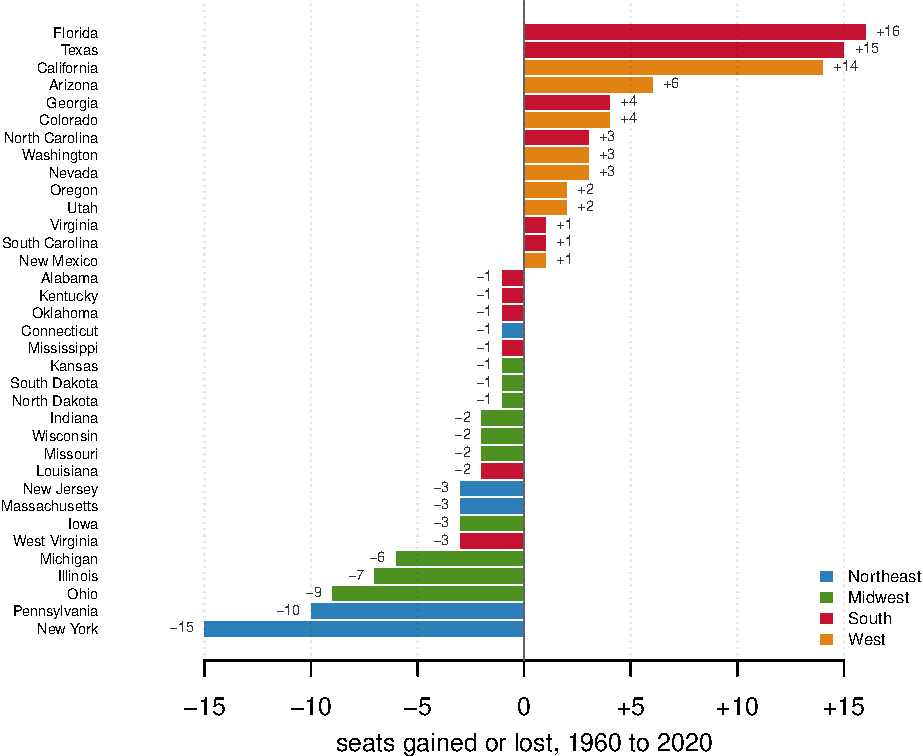
\includegraphics[keepaspectratio]{regional-shift-brief_files/figure-latex/bars-static-1.pdf}}

\textbf{Figure 1. The 35 states whose delegation changed size between
1960 and 2020.} One signed bar per state fits the question because the
question is who gained and who paid: bars right of the zero line took
seats, bars left of it gave them up, and color is Census region. Four
states take most of the gains: Florida +16, Texas +15, California +14
and Arizona +6. Four take most of the losses: New York -15, Pennsylvania
-10, Ohio -9 and Illinois -7.

\textbf{Both lists are geographically pure, and nobody arranged that.}
The gainers are Southern and Western, the losers Northeastern and
Midwestern, and no step in the procedure that produced them knows what a
region is. The formula sees fifty population counts.

{\def\LTcaptype{none} % do not increment counter
\begin{longtable}[]{@{}
  >{\raggedright\arraybackslash}p{(\linewidth - 8\tabcolsep) * \real{0.2941}}
  >{\raggedleft\arraybackslash}p{(\linewidth - 8\tabcolsep) * \real{0.1618}}
  >{\raggedleft\arraybackslash}p{(\linewidth - 8\tabcolsep) * \real{0.1618}}
  >{\raggedleft\arraybackslash}p{(\linewidth - 8\tabcolsep) * \real{0.1029}}
  >{\raggedleft\arraybackslash}p{(\linewidth - 8\tabcolsep) * \real{0.2794}}@{}}
\toprule\noalign{}
\begin{minipage}[b]{\linewidth}\raggedright
Region
\end{minipage} & \begin{minipage}[b]{\linewidth}\raggedleft
Seats 1960
\end{minipage} & \begin{minipage}[b]{\linewidth}\raggedleft
Seats 2020
\end{minipage} & \begin{minipage}[b]{\linewidth}\raggedleft
Change
\end{minipage} & \begin{minipage}[b]{\linewidth}\raggedleft
Share of the House
\end{minipage} \\
\midrule\noalign{}
\endhead
\bottomrule\noalign{}
\endlastfoot
Northeast & 108 & 76 & -32 & 24.8\% → 17.5\% \\
Midwest & 125 & 91 & -34 & 28.7\% → 20.9\% \\
South & 133 & 164 & +31 & 30.6\% → 37.7\% \\
West & 69 & 104 & +35 & 15.9\% → 23.9\% \\
Northeast + Midwest & 233 & 167 & -66 & 53.6\% → 38.4\% \\
South + West & 202 & 268 & +66 & 46.4\% → 61.6\% \\
\end{longtable}
}

The last column is worth reading slowly. \textbf{In 1960 the Northeast
and Midwest together held a majority of the House} --- 233 seats of 435.
They now hold 167, which is 38.4\% of it. A bloc that could pass a bill
on its own votes now cannot, and the loss of that majority was never on
any agenda. The presidential counterpart follows automatically, since
electors are seats plus two.

{\def\LTcaptype{none} % do not increment counter
\begin{longtable}[]{@{}lr@{}}
\toprule\noalign{}
Quantity & Value \\
\midrule\noalign{}
\endhead
\bottomrule\noalign{}
\endlastfoot
Northeast + Midwest electoral votes, 1960 & 275 of 535 (51.4\%) \\
Northeast + Midwest electoral votes, 2020 & 209 of 535 (39.1\%) \\
South + West electoral votes, 1960 & 260 of 535 (48.6\%) \\
South + West electoral votes, 2020 & 326 of 535 (60.9\%) \\
Electoral votes that changed region & 66 \\
\end{longtable}
}

The electoral-vote table is arithmetic about states, not a claim about
parties: this file has no election results in it, so nothing here says
who benefited.

\subsubsection{A ratchet, not a slosh}\label{a-ratchet-not-a-slosh}

There is an obvious objection. Seats bounce, and a state that gains
three in one decade and returns three in the next has moved nothing in
the end. If that is the story, 75 is churn rather than direction. The
file answers cleanly. Sum the per-decade columns, counting every seat
any state gained at any reapportionment: 78. The sixty-year total is 75.
The two can only differ by a state that gains a seat and later hands it
back, so the gap is a count of reversals, and it is 3.

{\def\LTcaptype{none} % do not increment counter
\begin{longtable}[]{@{}
  >{\raggedright\arraybackslash}p{(\linewidth - 6\tabcolsep) * \real{0.1528}}
  >{\raggedright\arraybackslash}p{(\linewidth - 6\tabcolsep) * \real{0.4583}}
  >{\raggedleft\arraybackslash}p{(\linewidth - 6\tabcolsep) * \real{0.1528}}
  >{\raggedleft\arraybackslash}p{(\linewidth - 6\tabcolsep) * \real{0.2361}}@{}}
\toprule\noalign{}
\begin{minipage}[b]{\linewidth}\raggedright
State
\end{minipage} & \begin{minipage}[b]{\linewidth}\raggedright
Seats, 1960 to 2020 by decade
\end{minipage} & \begin{minipage}[b]{\linewidth}\raggedleft
Net change
\end{minipage} & \begin{minipage}[b]{\linewidth}\raggedleft
Seats given back
\end{minipage} \\
\midrule\noalign{}
\endhead
\bottomrule\noalign{}
\endlastfoot
California & 38 → 43 → 45 → 52 → 53 → 53 → 52 & +14 & 1 \\
Montana & 2 → 2 → 2 → 1 → 1 → 1 → 2 & 0 & 1 \\
Tennessee & 9 → 8 → 9 → 9 → 9 → 9 → 9 & 0 & 1 \\
\end{longtable}
}

47 of the 50 states moved in one direction only across the whole period;
the 3 exceptions are the rows above, each accounting for exactly one
seat. This is not a cycle. It is a ratchet, and a ratchet does not have
to move quickly to end up somewhere a cycle never could.

\subsubsection{Since when}\label{since-when}

Seats arrive in whole-number jumps, so they lag the thing they measure.
Population share does not, and it reaches back to 1910.

\pandocbounded{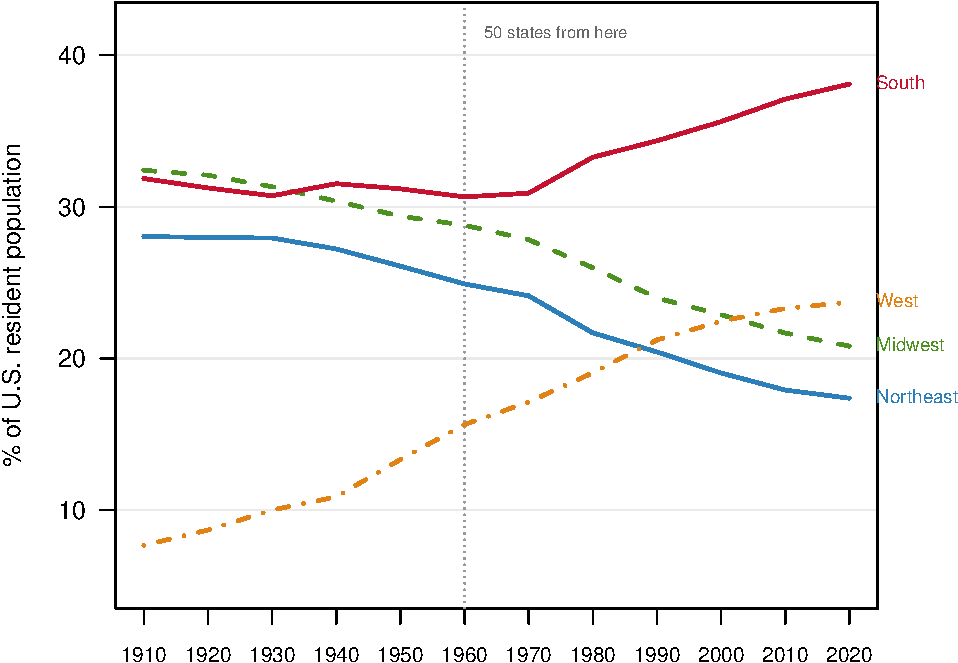
\includegraphics[keepaspectratio]{regional-shift-brief_files/figure-latex/lines-static-1.pdf}}

\textbf{Figure 2. Each Census region's share of the national population,
1910 to 2020.} A line per region fits the question because the question
is \emph{when}: a share that can be read at every census shows the
crossings that seat counts only echo a decade late. The dotted rule
marks 1960, the first apportionment with fifty states. The Northeast
falls the whole way, from 28.0\% to 17.4\%, the only region with no
reversal across 110 years. The West is the fastest thing on the chart,
rising from 7.7\% to 23.7\%; it passes the Northeast in 1990 and the
Midwest in 2010, and the South passes the Midwest in 1940.

The surprise is the South's timing. \textbf{The rise of the South does
not begin when the phrase suggests.} Between 1910 and 1960 the Census
South's share of the country actually \emph{fell}, from 31.9\% to
30.7\%, and the eleven-state Confederate South was flat. Everything the
phrase refers to happens after 1960. The window chosen because the
fifty-state House begins there turns out to be the right cut on the
substance as well, which is luck, and worth noticing as luck.

\subsubsection{Whether the South is eleven states or
seventeen}\label{whether-the-south-is-eleven-states-or-seventeen}

The most common objection to a regional finding is that the region is a
choice, and here it is easy to press, because there is no agreed answer
to what the South is. Political history usually means the eleven former
Confederate states. The Census Bureau means sixteen states plus the
District of Columbia. So compute the rise every way, with the disputed
states as a category of their own.

{\def\LTcaptype{none} % do not increment counter
\begin{longtable}[]{@{}
  >{\raggedright\arraybackslash}p{(\linewidth - 8\tabcolsep) * \real{0.5244}}
  >{\raggedleft\arraybackslash}p{(\linewidth - 8\tabcolsep) * \real{0.0854}}
  >{\raggedleft\arraybackslash}p{(\linewidth - 8\tabcolsep) * \real{0.1341}}
  >{\raggedleft\arraybackslash}p{(\linewidth - 8\tabcolsep) * \real{0.1341}}
  >{\raggedleft\arraybackslash}p{(\linewidth - 8\tabcolsep) * \real{0.1220}}@{}}
\toprule\noalign{}
\begin{minipage}[b]{\linewidth}\raggedright
Definition
\end{minipage} & \begin{minipage}[b]{\linewidth}\raggedleft
States
\end{minipage} & \begin{minipage}[b]{\linewidth}\raggedleft
Share 1960
\end{minipage} & \begin{minipage}[b]{\linewidth}\raggedleft
Share 2020
\end{minipage} & \begin{minipage}[b]{\linewidth}\raggedleft
Change
\end{minipage} \\
\midrule\noalign{}
\endhead
\bottomrule\noalign{}
\endlastfoot
Border South only (DC, DE, KY, MD, OK, WV) & 6 & 6.4\% & 5.5\% & -1.0
pts \\
Census South (16 states + DC) & 17 & 30.7\% & 38.1\% & +7.4 pts \\
Confederate South (11 states) & 11 & 24.2\% & 32.6\% & +8.4 pts \\
Northeast & 9 & 24.9\% & 17.4\% & -7.5 pts \\
Sun Belt (South + West) & 30 & 46.3\% & 61.8\% & +15.5 pts \\
\end{longtable}
}

\textbf{The narrower definition gives the larger rise.} The eleven
Confederate states gain 8.4 points of national population share; the
Census South, which contains all eleven and six units more, gains only
7.4. That is arithmetically possible only if the extra states are a
drag, and they are: Maryland, Delaware, Kentucky, Oklahoma, West
Virginia and the District went from 6.4\% of the country to 5.5\%.
Demographically they behave like the Northeast, whatever they are
called. The finding survives every version of the South in the table,
and the broadest version is the one that understates it.

\subsection{What this brief cannot tell
you}\label{what-this-brief-cannot-tell-you}

\textbf{This file cannot say why anybody moved.} It has population and
seats and nothing else: no births, no migration, no incomes, no housing
costs, no party labels. It cannot distinguish a family arriving in
Phoenix from Michigan from a family arriving from abroad, or either from
Arizona families simply being larger.

Nor can it certify the counts. The populations are printed as exact
whole numbers, and the Supreme Court's 1999 sampling decision makes them
exact as a matter of law, while the Bureau's own published coverage
estimates say they are not exact in fact. The margins here are large
enough that coverage error does not threaten them, since 15 seats is not
an error bar.

And the file is coarse. Twelve observations, one per decade, so anything
that happened between two censuses is invisible; four regions for fifty
states, with the South the most contested of them. Testing three
definitions of the South measures how much the finding depends on that
choice. It does not make the category natural.

\subsection{What you should have
learned}\label{what-you-should-have-learned}

\begin{itemize}
\tightlist
\item
  75 House seats changed states between 1960 and 2020, 66 of them
  crossing from the Northeast and Midwest to the South and West, with no
  vote taken anywhere.
\item
  The Northeast and Midwest held 233 of 435 seats in 1960, a majority of
  the House; they now hold 38.4\% of it.
\item
  The movement is a ratchet, not churn: 47 of 50 states travelled in one
  direction only, and the whole gap between the per-decade sums and the
  sixty-year total is 3 returned seats.
\item
  The claim survives every definition of the South, and the broadest
  definition produces the smallest rise, because the border states it
  adds shrank while the states below them grew.
\end{itemize}

\subsection{Extensions}\label{extensions}

\begin{itemize}
\tightlist
\item
  \texttt{southdefs.csv} defines the South four different ways and gives
  each a population and a share. Follow one definition across the years,
  then another. How much of ``the South is growing'' is a choice about
  which states you meant?
\item
  \texttt{seatchange.csv} has \texttt{reps\_1960} and
  \texttt{reps\_2020} for every state alongside \texttt{pop\_growth}.
  Sort by \texttt{change}. Do the states that gained the most seats
  always have the fastest growth?
\item
  \texttt{regions.csv} carries both \texttt{share} of population and
  \texttt{seat\_share}. Take the difference for each region and year.
  Does representation track population immediately, or lag behind it?
\item
  \texttt{states.csv} flags each state as \texttt{south\_census},
  \texttt{south\_confed}, \texttt{sunbelt} or \texttt{border\_south}.
  Find the states the labels disagree about. What is a regional label
  actually measuring?
\item
  \textbf{Stretch.} The Bureau publishes yearly components of population
  change --- births, deaths, and movement in and out --- for recent
  decades. Fetch one state's series and ask \emph{why} it grew, the
  question this file cannot answer.
\item
  \textbf{Stretch.} The Bureau also publishes the priority values behind
  each apportionment. Re-run the 2020 hand-out under a different divisor
  rule and ask how much of the shift is formula rather than migration.
\end{itemize}

\subsection{Sources}\label{sources}

\textbf{Data}

\begin{itemize}
\tightlist
\item
  U.S. Census Bureau, \emph{Apportionment Data (Text Version)},
  decennial apportionment time series 1910--2020.
  \url{https://www.census.gov/data/tables/time-series/dec/apportionment-data-text.html}
  Direct file:
  \url{https://www2.census.gov/programs-surveys/decennial/2020/data/apportionment/apportionment.csv}
\item
  U.S. Census Bureau, \emph{Statistical Groupings of States and
  Counties} (Geographic Areas Reference Manual, ch.~6), for the four
  regions and nine divisions.
\end{itemize}

\textbf{The data itself}

Every figure above is drawn from these tables. They are plain CSV, they
open in a spreadsheet, and they are yours to take further.

\href{data/derived/nation.csv}{\texttt{nation.csv}},
\href{data/derived/regions.csv}{\texttt{regions.csv}},
\href{data/derived/seatchange.csv}{\texttt{seatchange.csv}},
\href{data/derived/southdefs.csv}{\texttt{southdefs.csv}},
\href{data/derived/states.csv}{\texttt{states.csv}}

\textbf{Cases, statutes and literature}

\begin{itemize}
\tightlist
\item
  \emph{Department of Commerce v. United States House of
  Representatives}, 525 U.S. 316 (1999), holding that the Census Act
  forbids the use of statistical sampling to produce the population
  figures used for apportionment.
\item
  Permanent Apportionment Act of 1929, 46 Stat. 21.
\item
  Gaines, B. J. and Jenkins, J. A. (2009). ``Apportionment Matters: Fair
  Representation in the US House and Electoral College.''
  \emph{Perspectives on Politics} 7(4): 849--857.
\end{itemize}

\begin{ddaiprompt}{rebuild}{Rebuild this data yourself, with an AI assistant}
I want to rebuild a public dataset from its original source, without any
starting files. Please do the following and show your work.

THE SOURCE. U.S. Census Bureau, the apportionment time series: every
state's population and House seats at every census from 1910 to
2020, in one CSV of about 40 KB:
https://www2.census.gov/programs-surveys/decennial/2020/data/apportionment/apportionment.csv
No account or key is needed. One row is one geography in one census
year, and a "Geography Type" column says which kind: State (52 per
year -- the 50 states, DC and Puerto Rico), Region, or Nation. Three
things to survive. Every numeric column is a quoted string with
thousands separators, like "2,138,093" -- strip the commas before
any arithmetic, or every value over 999 silently becomes missing.
Alaska and Hawaii appear from 1910 with blank seat counts until
1960, because they were territories. And Puerto Rico is a State-type
row that is NOT in the national total, while DC is in the total and
has no seats.

WHAT TO BUILD.
1. A state-by-decade table of population and seats -- and a check:
   the State rows, summed with the cautions above, should reproduce
   the file's own Region and Nation rows exactly.
2. The nation per decade: population, House size, and people per
   seat.
3. Seat change from 1960 to 2020, state by state: who gained, who
   paid.

CHECK YOUR WORK. The copy this book used was fetched in August 2026.
If your rebuild matches it, you should find:
- 684 data rows
- the 2020 Nation row: 331,449,281 people, 435 seats, 761,169 people
  per seat
- 433 seats in the 1910 row, then 435 in every decade after
- from 1960 to 2020: Florida +16 seats, Texas +15, California +14
This series gains one decade per census; the next rows arrive with
the 2030 count, and nothing already in the file changes.
\end{ddaiprompt}

\end{document}
